\documentclass[11pt,a4paper]{article}
\usepackage[utf8]{inputenc}
\usepackage[T1]{fontenc}
\usepackage[french]{babel}
\usepackage{lmodern}
\usepackage{microtype}
\usepackage{geometry}
\geometry{margin=2.5cm}
\usepackage{graphicx}
\usepackage{float}
\usepackage[hidelinks]{hyperref}
\usepackage{listings}
\usepackage{amsmath}

\title{RAPPORT \\ Projet Audionumérique - Application de dessin sonore}
\author{Alexis Gaudray Bouju \\ Eve Turchet}
\date{Semestre 8 - 2025/2026}

\graphicspath{./img/}

\begin{document}
\maketitle
\renewcommand{\contentsname}{Table des matières}
\tableofcontents
\newpage

\section{Introduction}

Dans le cadre du projet d'audionumérique, nous avons exploré la relation entre la musique et le dessin.
L'objectif de ce projet était de créer une application qui permet de jouer du son en temps réel à partir d'un dessin de l'utilisateur sur une fenêtre graphique.
Le projet est disponible sur GitHub à l'adresse suivante : \url{https://github.com/Evemouth/audionum-projet}.

\section{L'application}

Notre application se décompose en trois parties principales : l'interface graphique présentée en section~\ref{sec:interface}, la génération du son détaillée en section~\ref{sec:son} et la création des grilles en section~\ref{sec:grilles}.

\subsection{L'interface graphique}
\label{sec:interface}

L'application que nous avons développée utilise la bibliothèque Pygame pour créer une interface graphique où l'utilisateur peut dessiner avec sa souris.
Sur la fenêtre graphique présentée en Figure~\ref{fig:interface}, nous affichons les informations relatives au fichier MIDI comme son nom, la première note du morceau ou encore les deux intervalles principaux. \\

En fond de l'interface, nous retrouvons une grille construite à partir du fichier MIDI qui sert de base à l'utilisateur pour la génération du son.
De cette manière, l'utilisateur peut repérer la première note du morceau au centre de la grille en rouge et se guider des axes pour créer des mélodies plus harmonieuses.\\

L'interface comporte également une palette de couleurs qui représente des instruments de musique différents.
Cela permet à l'utilisateur de découvrir différentes sonorités en mélangeant les couleurs dans son dessin.\\

Enfin, l'utilisateur a la possiblité de sauvegarder son dessin avec la touche \texttt{CTRL+S} ou de réinitialiser la fenêtre avec la touche \texttt{CTRL+Z}.

\begin{figure}[H]
    \centering
    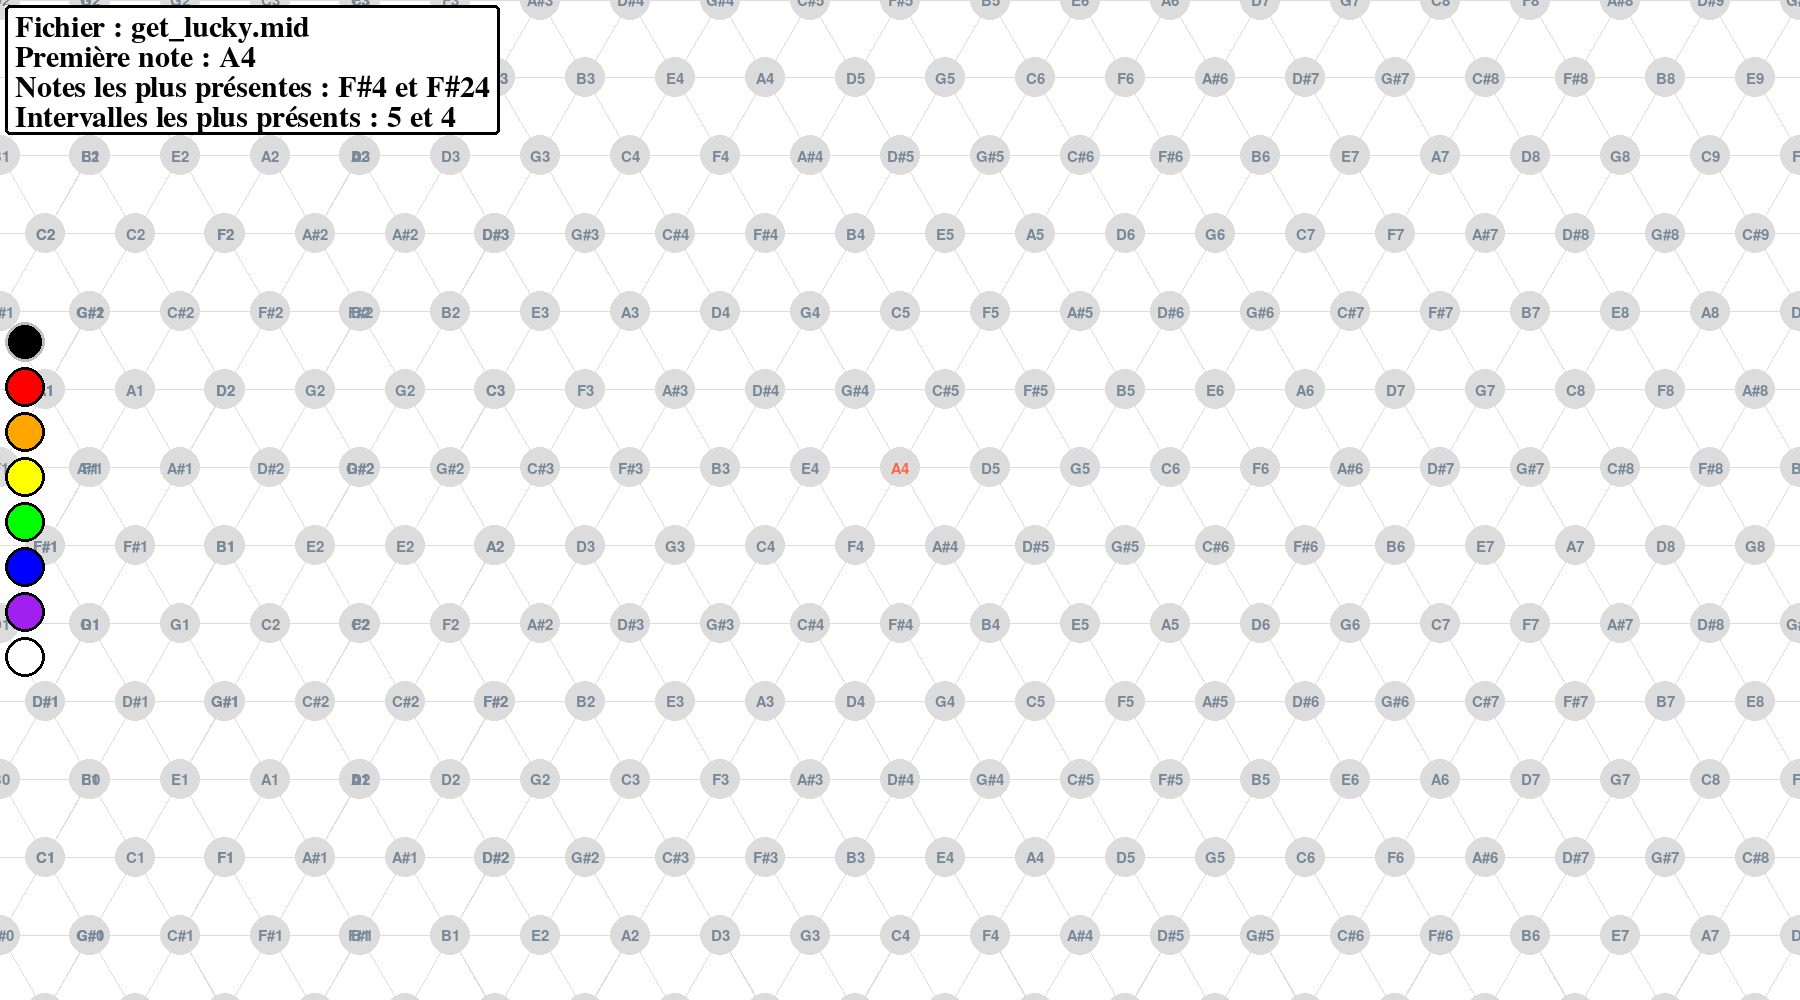
\includegraphics[width=0.49\textwidth]{img/grille_vide.png}
    \hfill
    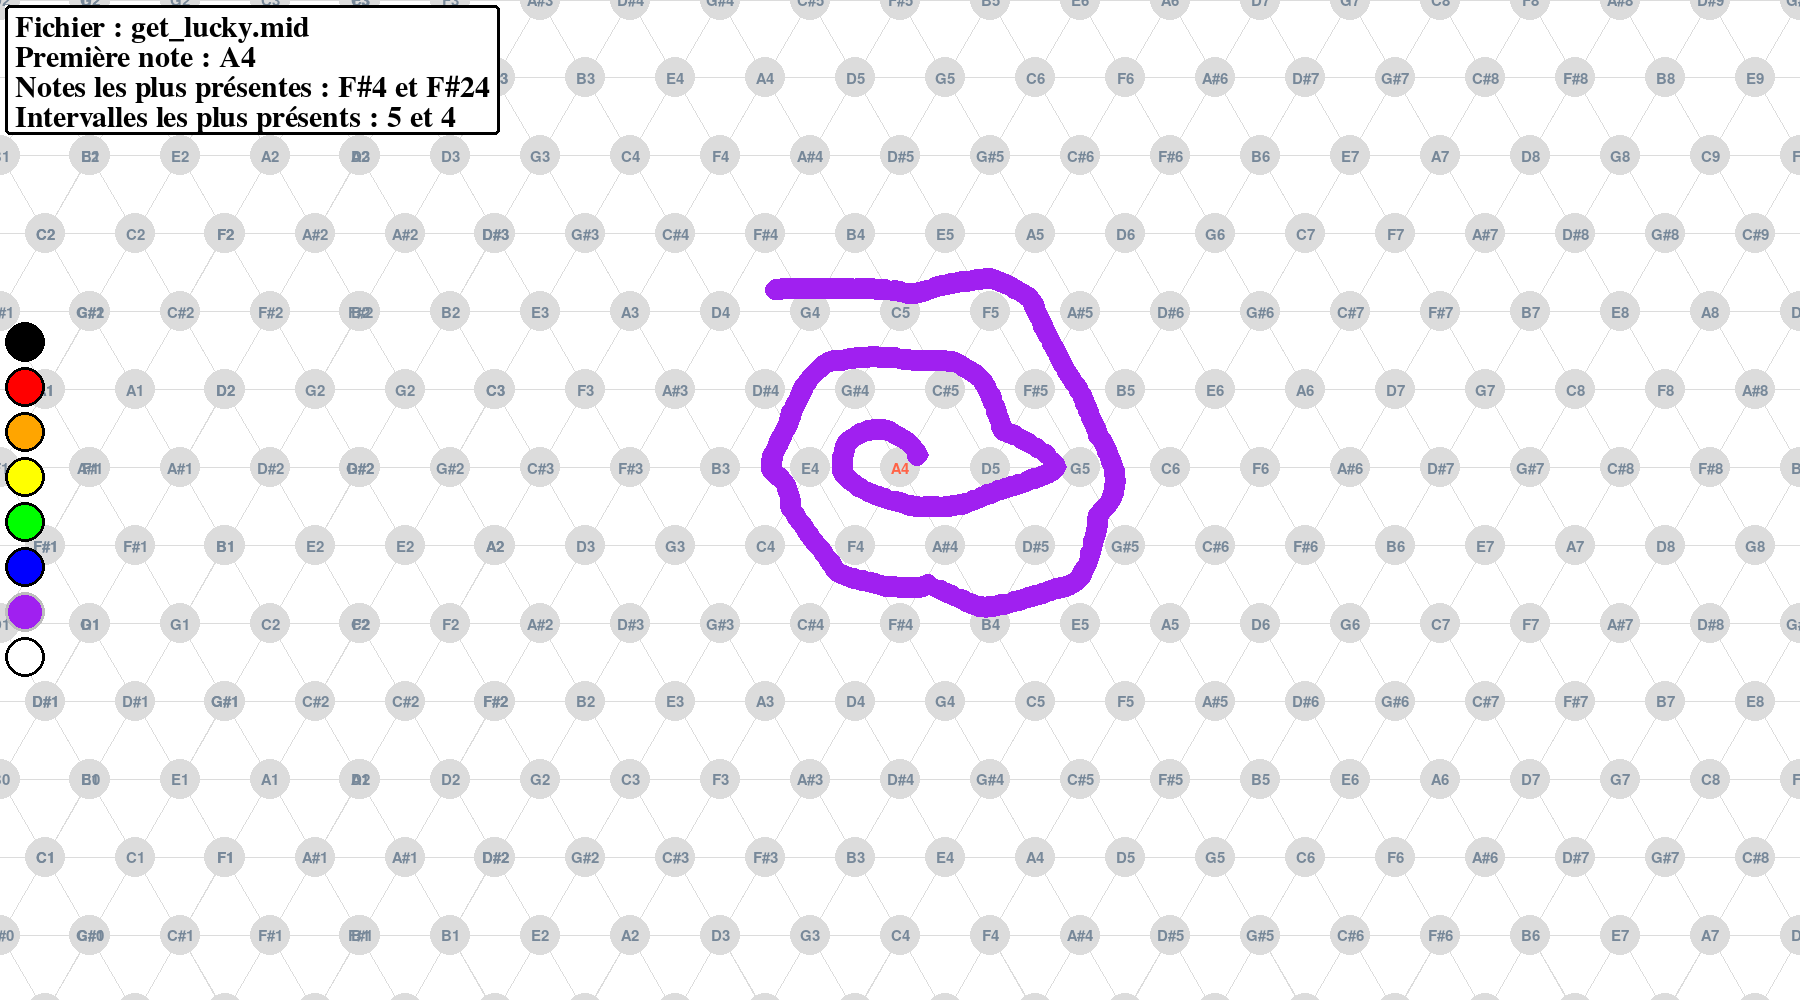
\includegraphics[width=0.49\textwidth]{img/grille_dessin.png}
    \caption{Interface graphique de l'application initiale (à droite) et avec un dessin réalisé par l'utilisateur (à gauche).}
    \label{fig:interface}
\end{figure}

\subsection{La génération du son}
\label{sec:son}

La première version de l'application générait du son de manière continue en fonction de la position du curseur sur la fenêtre graphique.
Dans cette première approche, nous calculions une fréquence à partir des coordonnées du curseur.
Nous partions d'une note de base (un \textit{La} à 440~Hz), et plus l'utilisateur déplaçait sa souris vers la droite ou vers le bas de l'écran, plus la note devenait aiguë.
Pour assurer un retour audio immédiat et fluide pendant le dessin, on envoyait un signal sonore court de manière répétitive.
Néanmoins, cela produisait un son peu mélodieux et peu agréable à l'écoute.\\

Nous avons ensuite décidé d'utiliser des notes au format MIDI pour générer des sons plus harmonieux.
La position horizontale (x) était convertie en une note dans la gamme \textit{["C", "C\#", "D", "D\#", "E", "F", "F\#", "G", "G\#", "A", "A\#", "B"]} tandis que la position verticale (y) donnait l'octave de la note.
Cette version donnait un résultat exploitable, mais se limitait à la reproduction d'un piano sous forme d'une grille rectangulaire.\\

Finalement, nous avons choisi de construire un système de grille avec différents pavages, générés à partir d'un fichier MIDI.
L'idée est d'adapter la disposition des notes du pavage en fonction d'une musique de référence, afin de créer un espace musical sur mesure.
Nous utilisons donc la bibliothèque \texttt{Mido} pour parcourir un fichier MIDI d'une musique et extraire la première note du morceau, la note la plus jouée et les deux intervalles les plus fréquents.
Cela permet de placer au centre du pavage la première note, et de graduer les différents axes avec les intervalles le plus fréquents.
Ainsi l'utilisateur peut rejouer la musique de départ facilement dans ce pavage en partant de la case centrale et en se déplaçant (de proche en proche la plupart du temps) sur les notes.

\subsection{Les grilles}
\label{sec:grilles}

Nous avons essayé plusieurs pavages avec des propriétés différentes, plus ou moins interressant musicalement.
Pour commencer, nous avons réalisé un pavage rectangulaire.
Dans ce pavage, chaque case correspond à une note MIDI : l'axe des abscisses est divisé en sept pour représenter les octaves et l'axe des ordonnées est séparé en douze pour représenter les notes de la gamme chromatique.
Cependant, ce pavage est vite limitant car il ne possède que deux axes.\\

Nous nous sommes donc ensuite dirigé vers le pavage triangulaire qui a l'avantage d'avoir un axe de plus en théorie.
En pratique, cet axe de plus est juste la combinaison des deux autres, donc pas réellement de possibilité supplémentaire.
L'inconvéniant de ce pavage est l'impossibilité de ce déplacer sur un même axe en cotinu.
En passant sur la base du triangle, on arrive ensuite sur un sommet, qui rend impossible le passage à son voisin sans toucher une autre case.\\

Nous nous sommes finalement tournés vers le pavage de combinaisons hexagonales pour introduire une nouvelle dimension en ajoutant des points aux sommets des hexagones.
Dans ce pavage inspiré de Tonnetz [\url{https://thetonnetz.com/}], les notes sont organisées de manière à ce que les intervalles harmoniques soient représentés par des déplacements simples sur la grille.
Par exemple, un déplacement vers la droite augmente la note d'un intervalle, un déplacement sur un axe diagonal augmente la note d'un deuxième intervalle et un déplacement sur la deuxième diagonale fait varier la note avec la somme des deux intervalles précédents.
Concernant la conception de ce pavage, nous avons enregistré tous les sommets et centres des hexagones puis nous leur avons associé une note à l'aide d'un parcours en largeur du graphe formé ainsi.

\section{Conclusion}

En conclusion, nous avons exploré la relation entre la musique et l'espace géométrique à travers le dessin.
Nous avons ainsi conçu un instrument de musique visuel et intuitif. \\

Pour donner suite au projet, plusieurs piste d'amélioration pourraient être envisagées.
En effet, il serait interressant de pouvoir changer de pavage depuis l'interface graphique et trouver quel pavage s'adapte le mieux à une musique.
Pour terminer, nous pourrions ajouter une fonctionnalité permettant de retracer un dessin en fonction d'un fichier MIDI. Actuellement, l'utilisateur peut sauvegarder le dessin final ainsi que le fichier MIDI généré de ce qu'il a joué (en faisant \texttt{Ctrl-S}) mais il serait également intéressant d'avoir la vidéo du traçage et du son généré en même temps.\\

\end{document}
